\begin{frame}{Abstract}
	In my M.Sc. project, I study the effects of the backreaction of a charged Klein-Gordon field coupled to an external electric field, in 1+1 dimensional spacetime.

In this talk, I motivate and state the problem I intend to solve, discuss existing results from the literature, and present preliminary results from my project.

\end{frame}

\section{Introduction}

\begin{frame}{Motivation}
	\begin{itemize}[<+->]
		\item \textbf{Historically} Vacuum polarization was one of the first quantum electrodynamical effects theoretically studied \cite{Uehl1935, Heis1936}.
		\item New interests in studying the effect of \textbf{boundary conditions} of QFT in the context of advanced materials  \cite{Fial2019}.
		\item \textbf{Toy model} for semi classical gravity. \cite{Wroc2011}
		\item  These calculations were \textbf{already done} \cite{Ambj1983}, but present counter intuitive results, such as anti-screening behavior for Neumann boundary conditions. These calculations were corrected by \cite{Wern2020}.
		\begin{enumerate}
			\item Use of a mode sum formula for the charge density
			\item Neglecting broken down modes for Neumann boundary conditions
		\end{enumerate}
\end{itemize}
	
\end{frame}

\begin{frame}{The problem}
		    \begin{figure}[ht]
		        \centering
		        \incfig{the-background-field-generated-by-two-opposite-charges-sitting-at-the-boundaries.}
		        \caption{the background field generated by two opposite charges sitting at the boundaries.}
		        \label{fig:the-background-field-generated-by-two-opposite-charges-sitting-at-the-boundaries.}
		    \end{figure}
\end{frame}

\begin{frame}{The problem}
\begin{figure}[ht]
    \centering
    \incfig{the-backreaction-of-the-klein-gordon-field.}
    \caption{The background electric field and the free Klein-Gordon field.}
    \label{fig:the-backreaction-of-the-klein-gordon-field.}
\end{figure}
\end{frame}

\begin{frame}{The problem}
\begin{figure}[ht]
    \centering
    \incfig{the-backreaction-of-the-klein-gordon-field2}
    \caption{The backreaction of the Klein-Gordon field}
    \label{fig:the-backreaction-of-the-klein-gordon-field}
\end{figure}
\end{frame}


\begin{frame}
    \begin{themedTitleBlock}{Semi classical Klein-Gordon-Maxwell equations}
	    \uncover<1->{
		    The goal is to solve the coupled system of equations\footnote{Notation: The metric signature is $(+,-)$ and the coordinates are  $x = (t, z)$}
	            \begin{align}
			    \begin{cases}
				    \left[ D_\mu D^\mu + m^2 \right] 	 \phi(x)= 0 
				    \\ 
				    \partial_\mu F^{\mu\nu} = \left<:j^{\nu}: \right>_{\phi} 
			    \end{cases}
		    \end{align}
		    \uncover<2->{
		        With the covariant derivative $$D_\mu = \partial_\mu + ieA_\mu,$$ } } \uncover<3->{
				\hspace{-0.3cm}and the boundary conditions
	        \begin{align}
	        	\begin{cases}
				\left . \hspace{0.14cm}\phi\hspace{0.9mm} \right|_{z=0, 1} &= 0 \\
					\left . E^{\phi} \right|_{z=0, 1} &= 0 
	        	\end{cases}
	        \end{align}
	    }
    \end{themedTitleBlock}
\end{frame}

\begin{frame}{The problem}
	\begin{center}
	\begin{tikzpicture}[
	    node distance=2cm,
	    main/.style = {draw, circle, minimum size=1.2cm, thick},
	    rect/.style = {draw, rectangle, minimum width=2.5cm, minimum height=1cm, thick},
	    every edge/.append style={-{Latex[scale=1.2]}, thick}
	]
	
	% Nodes
	\node[main] (KG) {$\phi$};
	\node[rect, right=2.7cm of KG] (Charge) {$\rho$};
	\node[rect, below=2.7cm of Charge] (Field) {$\vec{E}$};
	
	% Edges
	\draw[->] (KG) -- (Charge) node[midway, above] {Contributes to};
	\draw[->] (Charge) -- (Field) node[midway, right] {Interacts with};
	\draw[->] (Field) -- (KG) node[midway, left] {Influences};
	
	% Back reaction loop
	\path[->] (Field) edge [bend left=45] (KG);
	
	% Labels
	%\node[above] at (current bounding box.north) {Back Reaction with a Klein-Gordon Field in an External Electric Field};
	
	\end{tikzpicture}
	
\end{center}

\end{frame}

\section{Methods}

\begin{frame}{Fixing the gauge}
	\begin{columns}
	    \begin{column}{0.5\textwidth}
\begin{figure}[ht]
    \centering
    \incfig{the-background-classical-electric-field}
    \caption{The background electric field}
    \label{fig:the-background-classical-electric-field}
\end{figure}
	    \end{column}
	    \begin{column}{0.5\textwidth}
		    \begin{enumerate}[<+->]
		    	\item 
	    Constant electric field of strength $\lambda$ pointing towards positive $z.$
    \item Under the Coulomb gauge $$A_0(t, z) = -\lambda z,\, A_1(t, z) = 0$$ up to additive constant
    \item To ensure anti-symmetric solutions $$A_0(t, z)=-\lambda(z-\frac{1}{2})$$

		    \end{enumerate}
	    \end{column}
	\end{columns}

\end{frame}

\begin{frame}{Electromagnetic potential}
	\begin{columns}
	    \begin{column}{0.5\textwidth}
\begin{figure}[ht]
    \centering
    \incfig{the-background-classical-electric-field-and-potential}
    \caption{The background classical electric field and potential}
    \label{fig:the-background-classical-electric-field-and-potential}
\end{figure}
	    \end{column}
	    \begin{column}{0.5\textwidth}
		    \begin{enumerate}
		    	\item 
	    Constant electric field of strength $\lambda$ pointing towards positive $z.$
    \item Under the Coulomb gauge $$A_0(t, z) = -\lambda z,\, A_1(t, z) = 0$$ up to additive constant
    \item To ensure anti-symmetric solutions $$A_0(t, z)=-\lambda(z-\frac{1}{2})$$

		    \end{enumerate}
	    \end{column}
	\end{columns}
\end{frame}

\begin{frame}{Electromagnetic potential}
	\begin{columns}
	    \begin{column}{0.5\textwidth}
\begin{figure}[ht]
    \centering
    \incfig{the-background-electric-field-and-potential,-with-an-additional-(antisymmetric)-potential.}
    \caption{The background electric field and potential, with an additional (antisymmetric) potential.}
    \label{fig:the-background-electric-field-and-potential,-with-an-additional-(antisymmetric)-potential.}
\end{figure}
	    \end{column}
	    \begin{column}{0.5\textwidth}
		    \begin{enumerate}
		    	\item 
	    Constant electric field of strength $\lambda$ pointing towards positive $z.$
    \item Under the Coulomb gauge $$A_0(t, z) = -\lambda z,\, A_1(t, z) = 0$$ up to additive constant
    \item To ensure antisymmetric solutions 
    \begin{align*}
	    A_0(t, z)=&-\lambda(z-\frac{1}{2}) \\ &+ A_0^{\phi}(z)
    \end{align*}
		    \end{enumerate}
	    \end{column}
	\end{columns}
\end{frame}

\begin{frame}{The set up}
	\begin{themedTitleBlock}{Klein-Gordon equation}
		With the chosen gauge the KGM equations turn into
	\begin{align}
		( (\partial_t + ie A_0) ^2 - \partial_1^2+ m^2) \phi (x) &= 0,\\ 
		\partial_1 ^2 A_0^{\phi} &= - \left<\rho (z) \right>_\phi,
	\end{align}
with  
\begin{align}
	A_0 (z) &= -\lambda\left( z - \frac{1}{2} \right) + A_0^{\phi}(z), \\
	x &= (t, z) \in \R \times [0, 1]
\end{align}
	\end{themedTitleBlock}
\end{frame}

\begin{frame}{Time independent Klein-Gordon equation}
	\uncover<1->{
With the variable separation ansatz $\phi(x) = \phi_n(z)e^{-i\omega_n t}$,
	}
	\uncover<2->{
	\begin{themedTitleBlock}{Mode equation}
		For some potential $A_0(z)$
		\uncover<2->{
		    \begin{align}
		    	\left( \left[ \omega_n - eA_0(z)  \right]^2 + \frac{d^2}{d z ^2} + m^2  \right) \phi_n &= 0 
		    	\end{align}
		}
		Without backreaction
		\uncover<3->{
			\begin{align}
			\left( \left[ \omega_n + e\lambda \left(  z - \frac{1}{2}\right)  \right]^2 + \frac{d^2}{d z ^2}  + m^2\right) \phi_n &= 0
		\end{align}
		}
		
	\end{themedTitleBlock}
	}
\end{frame}

\begin{frame}{The external field approximation}
	Without taking backreaction into account, the KG equation can be solved by
\begin{align*}
	\phi_n(z) &= 
	a_n D_{i \frac{m^2}{2\lambda} - \frac{1}{2}} \left( 
		\frac{1+i}{\sqrt{\lambda} }
		\left( \omega_n + \lambda \left( z-\frac{1}{2} \right)
		\right) 
	\right) 
	\\
		  &+
	b_n D_{-i \frac{m^2}{2\lambda} - \frac{1}{2}} \left( 
		\frac{i - 1}{\sqrt{\lambda} }
		\left( \omega_n + \lambda \left( z-\frac{1}{2} \right)
		\right) 
	\right)
	\label{eq:parabolyc-cylinder}
\end{align*}
with $D_\nu(z)$ the parabolic cylinder functions.
\end{frame}

%\begin{frame}{The external field approximation -- Perturbation theory}
\uncover<1->{
	We want to turn the problem into a Schrödinger-like equation
	\begin{align}
		i\partial_t \ket{\Psi} = H\ket{\Psi}, 
		\text{with} \ket{\Psi} = \begin{pmatrix} \phi \\ \pi^* \end{pmatrix}, \,\text{and}\, \pi^* = D_0\phi
	\end{align}
}

\uncover<2->{
	The corresponding Hamiltonian would be 
	\begin{align}
		H = \underbrace{i \begin{pmatrix} 0 & 1 \\
		D_1^2 -m^2 & 0 
	\end{pmatrix}}_{H_0}+
	\underbrace{			\begin{pmatrix} eA_0 & 0 \\
				0 & eA_0
		\end{pmatrix}}_{H_1}.
	\end{align}
}
\uncover<3->{
Which is hermitean w.r.t. 
\begin{align}
	\bra{\Psi_1}\ket{\Psi_2} = i \int_{0}^{1} dz \left( \phi_1^{*}\pi_2^* -  \pi_{1} \phi_2 \right)  
\end{align}
}
\end{frame}

\begin{frame}{The external field approximation -- Perturbation theory}
	\uncover<1->{
		Eigenstates for $H_0$ given by 
		\begin{align}
			\omega_n = \text{sgn}(n) \sqrt{m^2 + n^2 \pi^2} , \hspace{0.5cm} \phi_n(z) = \frac{1}{\sqrt{\omega_n} } \sin(n\pi z)
		\end{align}
	}
	\uncover<2->{
		Calculate the first order corrections 
	    \begin{align}
	    	\omega_n ^{(1)} &= \frac{\bra{\Psi_n^{(0)}}\ket{H_1\Psi_n^{(0)}}}{\bra{\Psi_n^{(0)}}\ket{\Psi_n^{(0)}}} \\
	    	\ket{\Psi_n ^{(1)}} &= \sum_{k\neq n}^{} 
	    	\frac{
	    		1
	    	}
	    	{
	    	\bra{\Psi_n^{(0)}}\ket{\Psi_n^{(0)}}
	    	}
	    	\frac{
	    	\bra{\Psi_k^{(0)}}\ket{H_1\Psi_n^{(0)}}
	    	}{
	    	\omega_n ^{0} - \omega_k^{(0)}
	    	} \ket{\Psi_k^{(0)}}
	    \end{align}
	}
	
\end{frame}
\begin{frame}{The external field approximation -- Perturbation theory}
	\uncover<1->{
		Corrections to first order in $\lambda$
	\begin{align}
		\omega_n &= \text{sgn(n)}\sqrt{m^2 + n^2\pi^2}  \\
		\begin{split}
			\phi_n^{D} &= \left( m^2 + \pi^2  n^2 \right)^{-\frac{1}{2}} \left[ \sin\pi n z \right.\\
				   &\left.+ \lambda \frac{\sqrt{m^2 + \pi^2 n^2} }{2 \pi \lvert n \rvert} 
				\left( 
				\frac{1}{\pi n}\left( \frac{1}{2} - z \right) \sin \pi n z - z(1-z) \cos \pi n z \right) 
			\right] 
		\end{split}
	\end{align}
	}

\end{frame}


\begin{frame}{The external field approximation limitations}
	Results by  \cite{Ambj1983}:
	\begin{columns}
		\uncover<1->{
		    \begin{column}{0.5\textwidth}
		    \begin{figure}[h]
		    	\centering
		    	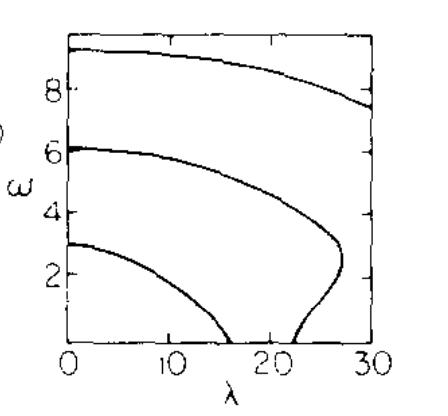
\includegraphics[width=0.5\textwidth]{figures/omega_wolfram.jpeg}
			\caption{Positive energy levels for increasing $\lambda$ \textbf{without} considering the backreaction of the massless Klein-Gordon field.}
		    	\label{fig:figures-omega_wolfram-jpeg}
		    \end{figure}
		    \end{column}
		    
		}
		
		\uncover<3->{

	    \begin{column}{0.5\textwidth}
	   \begin{figure}[h]
	   	\centering
	   	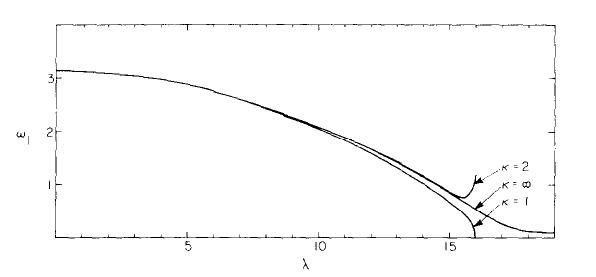
\includegraphics[width=0.9\textwidth]{figures/omega_backreaction.jpeg}
		\caption{Positive energy levels for increasing $\lambda$ \textbf{with} backreaction.}
	   	\label{fig:figures-omega_backreaction-jpeg}
	   \end{figure} 

	    \end{column}
		}
	\end{columns}
\end{frame}

%\begin{frame}{The exter}
%%	\begin{tikzpicture}
\begin{axis}[
    domain=0:1, % Adjust the domain as needed
    samples=100,
    xlabel={$z$},
    ylabel={$\phi_n^D$},
    legend pos=outer north east,
    grid=major
]

% Define the parameters
\pgfmathsetmacro{\m}{10}
\pgfmathsetmacro{\n}{1}
\pgfmathsetmacro{\piVal}{3.1415926}
\pgfmathsetmacro{\lambda}{20}

% Define the function f(z)
\pgfmathdeclarefunction{f}{1}{%
    \pgfmathparse{
        (1 / sqrt(\m^2 + \piVal^2 + \n^2)) * (
            sin(\piVal * \n * #1) +
            \lambda * sqrt(\m^2 + \piVal^2 * \n^2) / (2 * \piVal * abs(\n)) * (
                (1 / (\piVal * \n)) * (0.5 - #1) * sin(\piVal * \n * #1) -
                #1 * (1 - #1) * cos(\piVal * \n * #1)
            )
        )
    }%
}
% Define the function
\addplot[
    blue,
    thick,
    smooth
] 
    %expression{1 / sqrt(sqrt(\m^2 + \piVal^2 *\n^2)) * (sin(\piVal * \n * x) + \lambda * sqrt(\m^2 + \piVal^2 * \n^2) / (2 * \piVal * abs(\n)) * (1 / (\piVal * \n) * (0.5 - x) * sin(\piVal * \n * x) - x * (1 - x) * cos(\piVal * \n * x)))};
expression{f(x)}

\legend{$\phi_n^D(z)$}
\end{axis}
\end{tikzpicture}

%\end{frame}

\begin{frame}{Quantization and renormalization}
We quantize the field based on the mode solutions 
\begin{align}
	\phi(t, z) = \sum_{n>0}^{} a_n \phi_n(z) e^{-i\omega_nt}
	+\sum_{n<0}^{} b_n^{\dagger} \phi_n(z) e^{-i\omega_nt},
\end{align}
with $a_n$, $b_n$ the operators fulfilling 
\begin{align}
	\left[ a_n, a_m^\dagger \right] = \delta_{nm}, \hspace{1cm}
	\left[ b_n, b_m^\dagger \right] = \delta_{nm}, \\
	\left[ a_n, a_m\right] =\left[ a_n, b_m\right] =\left[ a_n, b_m^\dagger\right] =\left[ b_n, b_m\right] = 0 .
\end{align}
This also defines the vacuum by
\begin{align}
	a_n \ket{0} = b_n \ket{0}  = 0	
\end{align}

\end{frame}

\begin{frame}{Charge density}
	\uncover<1->{
		We calculate the \textbf{charge density} as the 0th component of the charge current 
	\begin{align}
		\rho(z) = ie\bra{0} \phi^*(z) D_0 \phi(z) - \phi(z) D_0 \phi^*(z) \ket{0}
	\end{align}
	}
	
	\uncover<2->{
	Ambj\o rn and Wolfram calculate it as one naïvely would, 
	\begin{align}
		\rho(z) = e\left( \sum_{n>0}^{} (\omega_n - eA_0(z)) \lvert \phi_n(z)  \rvert ^2+ \sum_{n<0}^{} (\omega_n - eA_0(z)) \lvert \phi_n(z) \rvert^2 \right) 
	\end{align}
	}
\end{frame}

\begin{frame}{Hadamard states and point-splitting}

	\uncover<1->{
	Assume that the state is of Hadamard form,
	\begin{align}
		w^{\phi \phi^*}_\Omega(x, x') = \bra{\Omega}\phi(x) \phi^*(x')\ket{\Omega}  = H^{\phi \phi^*}(x, x')+ R_\Omega^{\phi \phi^*}(x, x'),
	\end{align}
}
\uncover<2->{
	with 
	\begin{align}
		H^{\phi \phi^*}(x, x') = -\frac{1}{4\pi} U(x, x') \log(-(x-x')^2 + i\epsilon (x-x')^{0})
	\end{align}
	and $$U(x,x') = \exp\left( -i \int_{0}^{1}A_\mu ( x' + s(x-x')) (x-x')^\mu ds   \right).$$
	}
	
	\uncover<3->{
	Define the product of derivatives of fields as 
	\begin{align}
		\bra{\Omega} D_\alpha\phi(x)(D_\beta\phi)^*(x)\ket{\Omega} =
		\lim_{x'\to x} \left[ D_\alpha D'_\beta^*\left( 
		w^{\phi \phi^*}_\Omega(x, x') - H^{\phi \phi^*}(x, x')
		\right)  \right],
	\end{align}
	}

\end{frame}

\begin{frame}{Renormalizing charge densities}
	\uncover<1->{
	Recall the mode decomposition of the field
\begin{align}
	\phi(t, z) = \sum_{n>0}^{} a_n \phi_n(z) e^{-i\omega_nt}
	+\sum_{n<0}^{} b_n^{\dagger} \phi_n(z) e^{-i\omega_nt},
\end{align}
	the expression for charge density 
	\begin{align}
		\rho(x) = ie\bra{0} \phi^*(x) D_0 \phi(x) - \phi(x) D_0 \phi^*(x) \ket{0}, \hspace{0.1cm}D_0 = \partial_0 + ie A_0,
	\end{align}
	}
	\uncover<2->{
	Realizing the point splitting in the time direction $x' = (t+\tau, z)$, we calculate 
	\begin{align}
		\bra{0} \phi^*(x) D_0 \phi(x') \ket{0}= -i\sum_{n<0}^{} (\omega_n - eA_0(z)) \lvert \phi_n(z)  \rvert ^2e^{-i\omega_n(\tau +i\epsilon)}  
	\end{align}
	}
	
\end{frame}
\begin{frame}{Renormalizing charge densities}
	\uncover<1->{
	\begin{align}
		\bra{0} \phi^*(x) D_0 \phi(x') \ket{0}= -i\sum_{n<0}^{} (\omega_n - eA_0(z)) \lvert \phi_n(z)  \rvert ^2e^{-i\omega_n(\tau +i\epsilon)}  
	\end{align}
	}
	\uncover<2->{
	\begin{align}
		\bra{0} \phi(x) D_0^* \phi^*(x') \ket{0}= i\sum_{n>0}^{} (\omega_n - eA_0(z)) \lvert \phi_n(z)  \rvert ^2e^{i\omega_n(\tau +i\epsilon)}  
	\end{align}
	}
	\uncover<3->{
	\begin{align}
		D_0' H^{\phi \phi^*}(x, x')= -\frac{1}{2\pi} \frac{1}{\tau+ i\epsilon} U(x',x)+ \mathcal{O}(\tau) =  -\frac{1}{2\pi} \left( \frac{1}{\tau + i\epsilon} -ieA_0 \right) + \mathcal{O}(\tau)
	\end{align}
	}
	\uncover<4->{
	\begin{align}
		D_0'^* H^{\phi^* \phi}(x, x')= -\frac{1}{2\pi} \frac{1}{\tau+ i\epsilon} U(x,x')+ \mathcal{O}(\tau) =  -\frac{1}{2\pi} \left( \frac{1}{\tau + i\epsilon} +ieA_0 \right) + \mathcal{O}(\tau)
	\end{align}
	}
\end{frame}

\begin{frame}{The renormalized charge density}
	\uncover<1->{
	    \begin{align}
	    	\begin{split}
	    		\rho(z) = e \lim_{\tau \to 0}&\left( 
	    			 \sum_{n>0}^{} (\omega_n - eA_0(z)) \lvert \phi_n(z)  \rvert ^2e^{i\omega_n(\tau +i\epsilon)}  
				+\sum_{n<0}^{} (\omega_n - eA_0(z)) \lvert \phi_n(z)  \rvert ^2e^{-i\omega_n(\tau +i\epsilon)} 
	    		\right) \\
	    		&+ \frac{e^2}{\pi}A_0(z)
	    	\end{split}
	    \end{align}
	}
	\uncover<2->{
	\begin{align}
		\rho(z) = e\left( \sum_{n>0}^{} (\omega_n - eA_0(z)) \lvert \phi_n(z)  \rvert ^2+ \sum_{n<0}^{} (\omega_n - eA_0(z)) \lvert \phi_n(z) \rvert^2 \right) 
	\end{align}
	}
\end{frame}

%\begin{frame}{Computing the charge density}
%	\uncover<1->{
%	    \begin{align}
%	    	\begin{split}
%	    		\rho(z) = e \lim_{\tau \to 0}&\sum_{n>0}^{}\left( (\omega_{-n} - eA_0(z)) \lvert \phi_{-n}(z)  \rvert ^2e^{-i\omega_{-n}(\tau +i\epsilon)} 
%	    			+ (\omega_n - eA_0(z)) \lvert \phi_n(z)  \rvert ^2e^{i\omega_n(\tau +i\epsilon)}  
%	    		\right) \\
%	    		&+ \frac{e^2}{\pi}A_0(z)
%	    	\end{split}
%	    \end{align}
%	}
%	
%	\uncover<2->{
%In the chosen gauge with $\omega_{-n} =-\omega_n$	    
%	    \begin{align}
%	    	\begin{split}
%	    		\rho(z) = e \lim_{\tau \to 0}&\sum_{n>0}^{} \left(-(\omega_{n} + eA_0(z)) \lvert \phi_{-n}(z)  \rvert ^2
%				+ (\omega_n - eA_0(z)) \lvert \phi_n(z)  \rvert ^2\right)e^{i\omega_n(\tau +i\epsilon)  }
%	    		\\
%	    		&+ \frac{e^2}{\pi}A_0(z)
%	    	\end{split}
%	    \end{align}
%	}
%	
%	
%\end{frame}

%\begin{frame}{Computing the charge density}
%	    \begin{align}
%	    	\begin{split}
%	    		\rho(z) = e &\sum_{n=1}^{N} \left(-(\omega_{n} + eA_0(z)) \lvert \phi_{-n}(z)  \rvert ^2
%				+ (\omega_n - eA_0(z)) \lvert \phi_n(z)  \rvert ^2\right)  
%	    		\\
%	    		&+ \frac{e^2}{\pi}A_0(z)
%	    	\end{split}
%	    \end{align}
%	    \textcolor{red}{Note:} The cut-off at a finite $N$ yields an oscillatory charge density of period $\Delta z = \frac{1}{N+1}$. Needs averaging!
%\end{frame}
%
\begin{frame}{The renormalized charge density}
	\begin{columns}
	    \begin{column}{0.5\textwidth}
	    	    \begin{figure}[h]
	    	    	\centering
	    	    	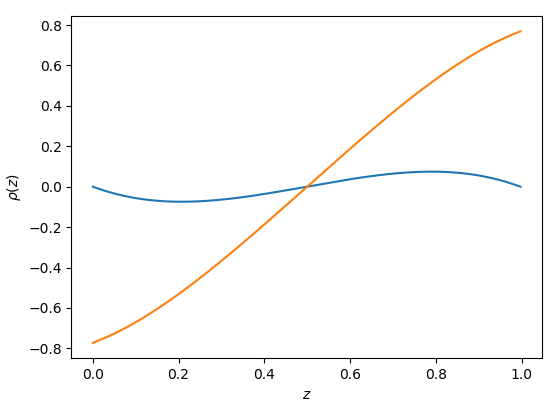
\includegraphics[width=0.9\textwidth]{figures/renormalization_comparison_rho.png}
	    	    \end{figure}
	    \end{column}
	    \begin{column}{0.5\textwidth}
		    The induced charge density $\rho$ resulting from the two different renormalization techniques with Dirichlet boundary conditions. $m=0$, $\lambda=5$.
		    \begin{itemize}
		    	\item \textcolor{orange}{In orange}, the charge density $\rho$ calculated through the mode sum formula.
			\item \textcolor{blue}{In blue}, the charge density $\rho$ calculated through Hadamard point-splitting. 
		    \end{itemize}
		    
	    \end{column}
	\end{columns}
	    \end{frame}

\begin{frame}{The induced fields}
	\begin{columns}
		\uncover<1->{
		        \begin{column}{0.5\textwidth}
		    	    The induced electric field:
		    	    \begin{align}
		    	    E^{\phi}(z) = \int_{0}^{z} \rho(z')dz' 
		    	    \end{align}
		        \begin{figure}[h]
		        	\centering
		        	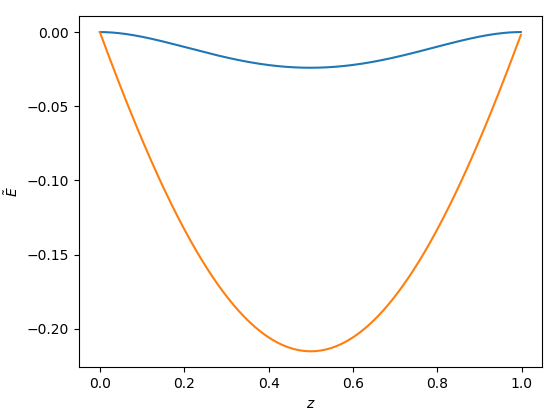
\includegraphics[width=0.8\textwidth]{figures/renormalization_comparison_induced_E.png}
		        \end{figure}
		        \end{column}
		}
		
		\uncover<2->{
		    
	    \begin{column}{0.5\textwidth}
		    	    The induced electric potential
		    	    \begin{align}
	A_0^{\phi}(z) = -\int_{0}^{z} E^{\phi}(z') dz'
		    	    \end{align}
		        \begin{figure}[h]
		        	\centering
		        	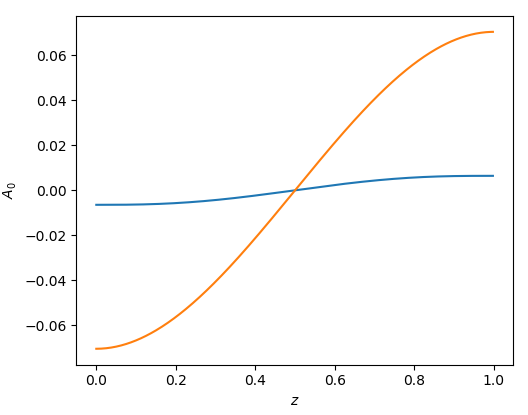
\includegraphics[width=0.8\textwidth]{figures/renormalization_comparison_induced_A0.png}
		        \end{figure}
		        \end{column}
		}
	\end{columns}
	\begin{centering}
		\hspace{2cm} \textcolor{orange}{In orange,} Mode sum. \textcolor{blue}{In blue,} Hadamard point-splitting.
	\end{centering}
\end{frame}

\begin{frame}{Closing the loop}
		
\begin{tikzpicture}[
    box/.style = {draw, rectangle, minimum width=2cm, minimum height=1cm},
    arrow/.style = {->, thin, >=Stealth},
    curved arrow/.style = {->, thick, >=Stealth, bend left}
]
\begin{centering}
	

% Nodes
\node[box] (A0) {$A_0^{(\kappa=0)}$};
\node[box, right=1cm of A0] (phi) {$\phi$};
\node[box, above right=1cm and 2cm of phi] (rho) {$\rho$};
\node[box, below right=1cm and 2cm of phi] (tildeA0) {$A^{\phi}_0^{\left( \kappa \right) }$};

% Curved arrows for the loop
\draw[arrow] (A0) -- (phi);
\draw[curved arrow, red] (phi) to[out=45, in=135] (rho);
\draw[curved arrow, red] (rho) to[out=45, in=135] (tildeA0);
\draw[curved arrow, red] (tildeA0) to[out=45, in=135] (phi);

% Center arrow with text
\node[right=0.9cm of phi] (kappa) {$\kappa \to \infty$};
 \draw[arrow, blue] (6.5, -0.25) arc [start angle=345, end angle=15, radius=1cm];


\end{centering}\end{tikzpicture}

\end{frame}

\begin{frame}{Closing the loop}

\begin{align}
			\left(
				\left[ 
			\omega^{\left( \kappa+1 \right) }_n 
	+ \lambda \left( z - \frac{1}{2} \right) 
- \left( A_0^{\phi} \right) ^{\left(\kappa  \right) }(z)  \right]^2 
	+ \frac{d^2}{dz^2} + m^2  \right)
	\phi^{\left( \kappa + 1 \right) }_n &= 0 \\
	\left(A_0^{\phi}  \right) ^{(\kappa)}(z) = -\int_{0}^{z} \int_{0}^{z'} \rho^{(\kappa)}(z'')dz''   dz'
,
\end{align}
\end{frame}

\begin{frame}{Visualizing the impact of backreaction}
	\begin{figure}[h]
		\centering
		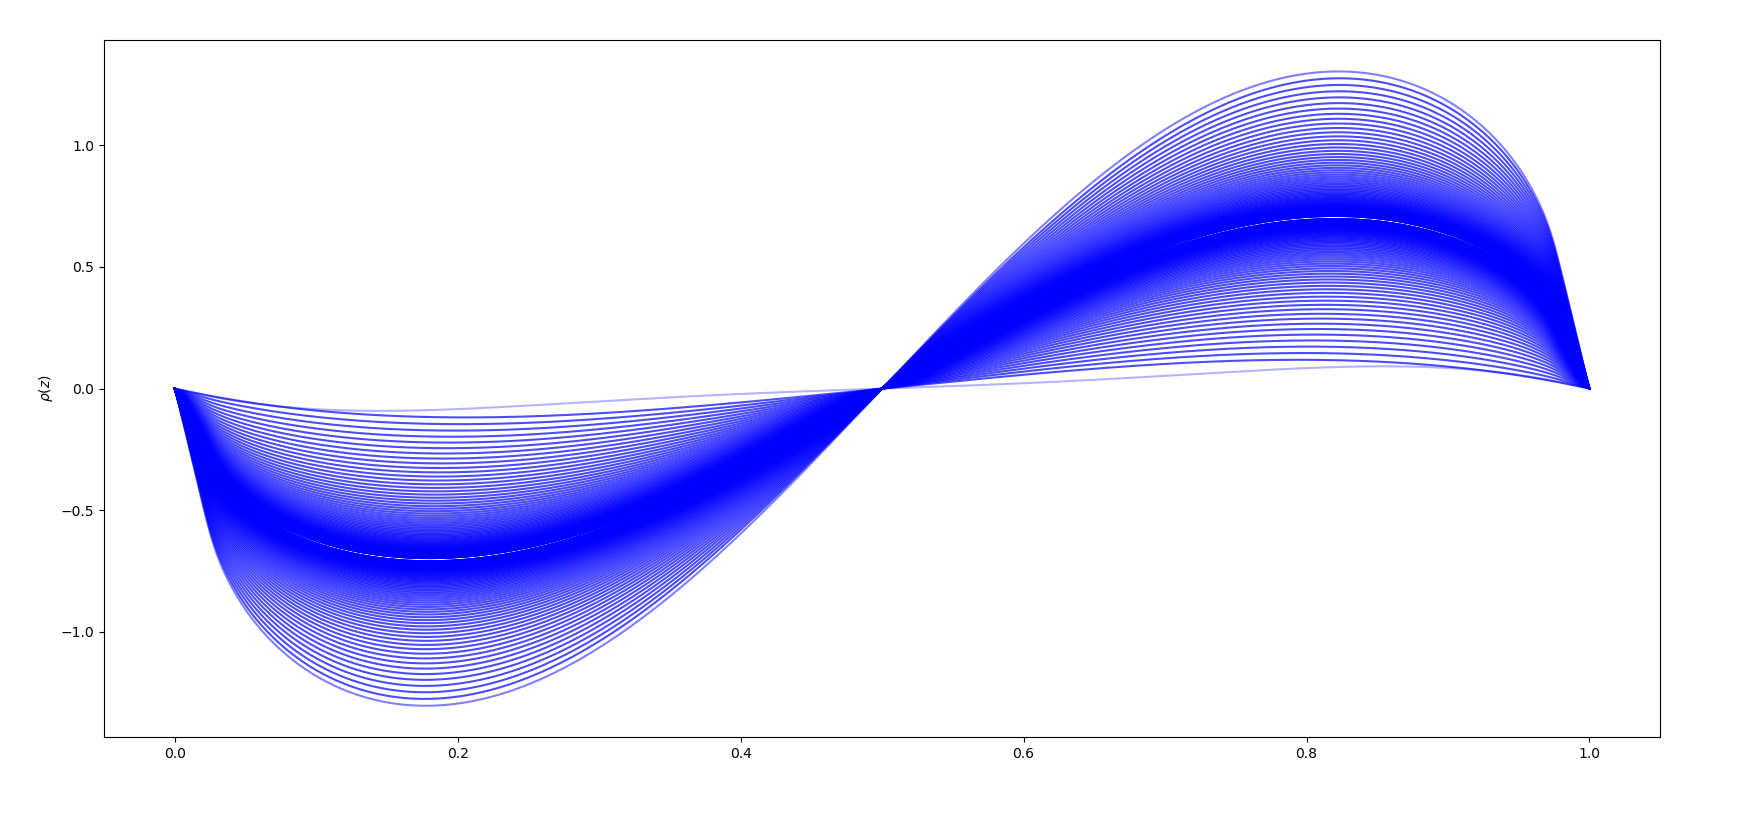
\includegraphics[width=0.7\textwidth]{figures/convergence_to_rho_a_10_0.png}
		% 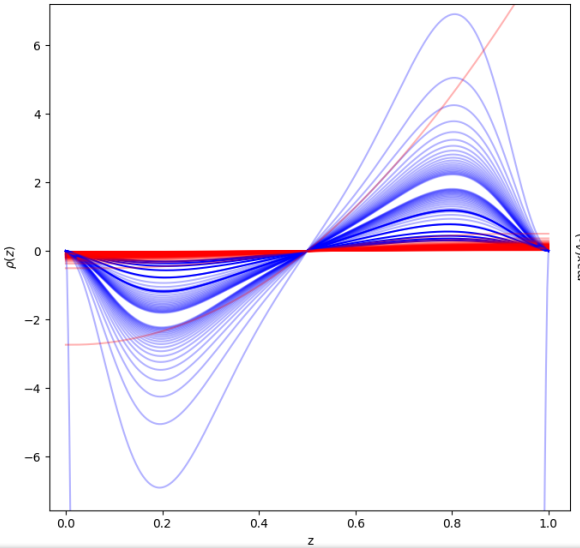
\includegraphics[width=0.4\textwidth]{figures/impact-of-backreaction.png}
		\caption{The convergence of $\rho^{\kappa}(z)$ as $\kappa\to \infty$ for $m=0$, $\lambda=15.5$.}
		\label{fig:figures-impact-of-backreaction-png}
	\end{figure}

\end{frame}

\section{Preliminary results}

\begin{frame}{$\omega_n$ dependence on $\lambda$ considering backreaction}
	\begin{figure}[h]
		\centering
		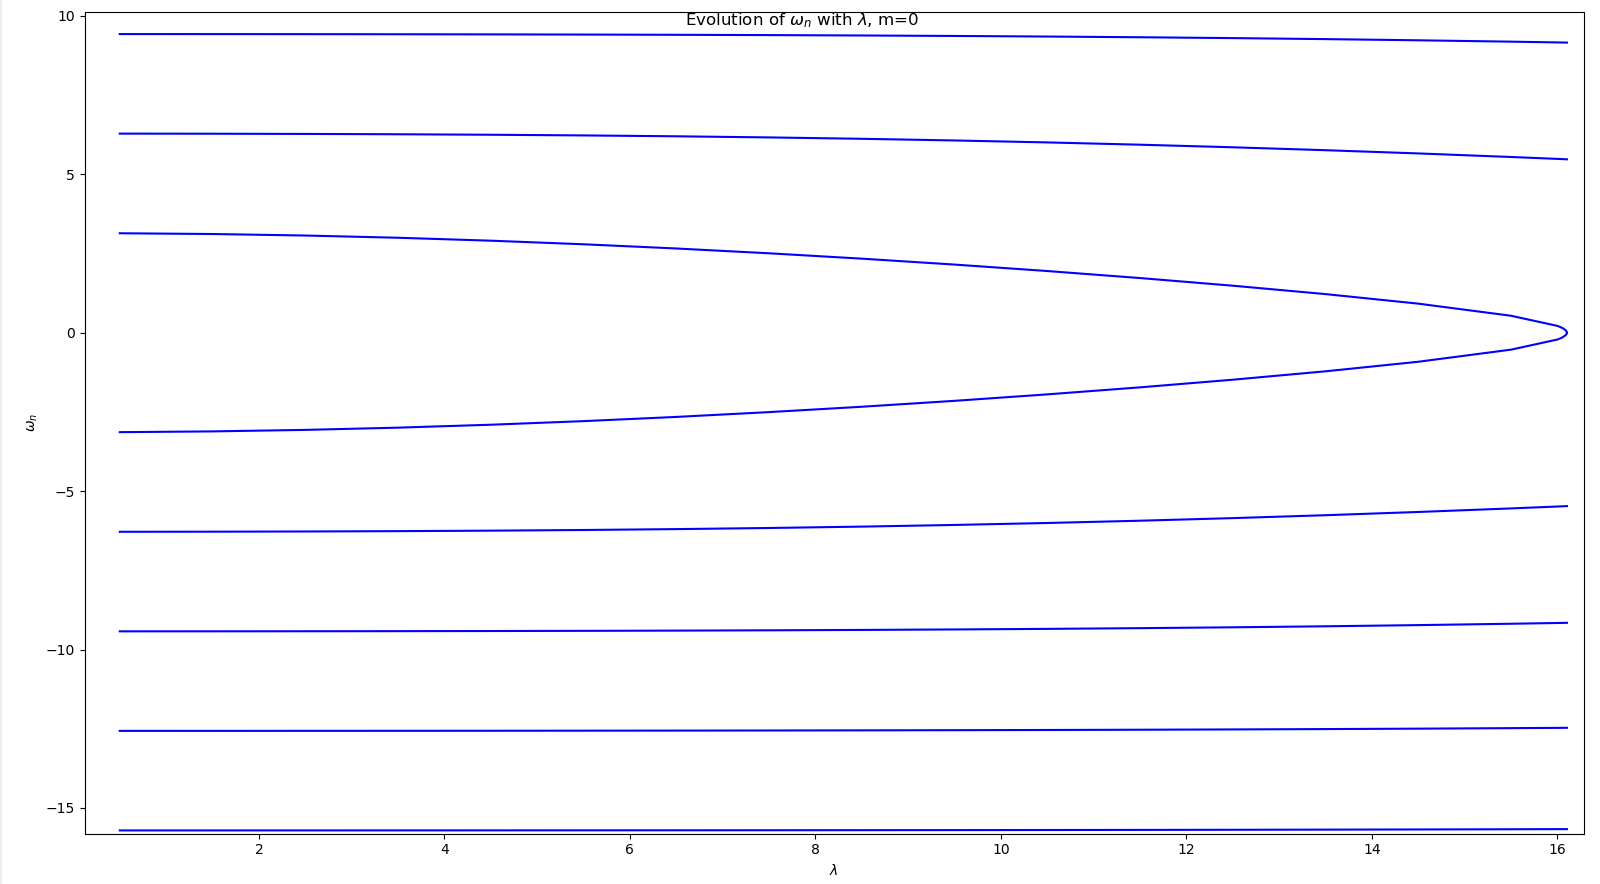
\includegraphics[width=0.8\textwidth]{figures/eigenvalue_evolution_a_1_0.png}
		\caption{$\omega_n$ as a function of $\lambda$ for the massless case.}
		\label{fig:figures-eigenvalue_evolution_a_1_0-png}
	\end{figure}

\end{frame}

\begin{frame}{Charge densities and $E^{\phi}$}
	\begin{columns}
	    \begin{column}{0.5\textwidth}
	    \begin{figure}[htpb]
	    	\centering
	    	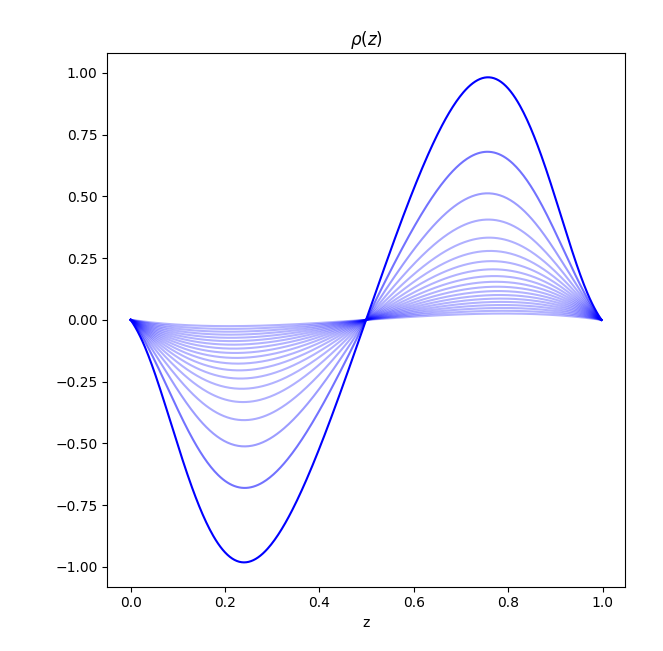
\includegraphics[width=0.8\textwidth]{figures/charge-density.png}
	    	\caption{Charge densities $\rho$ for increasing background electric field $\lambda$}
	    	\label{fig:figures-charge-density-png}
	    \end{figure}
	    \end{column}

	    \begin{column}{0.5\textwidth}
	    \begin{figure}[h]
	    	\centering
	    	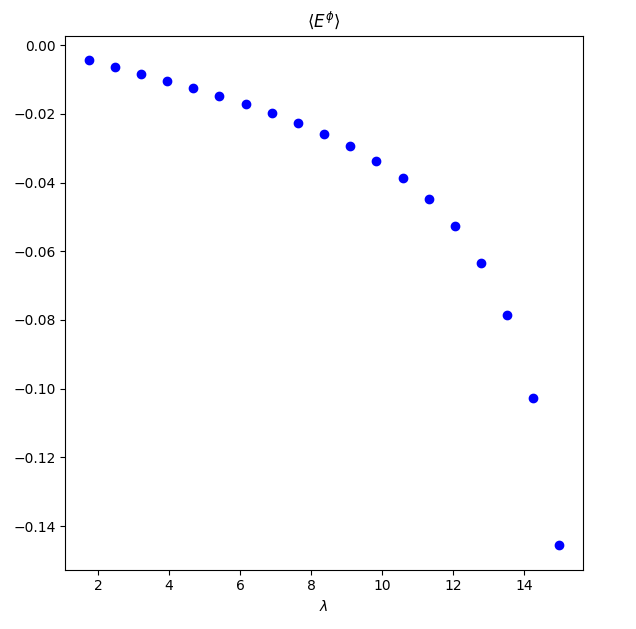
\includegraphics[width=0.8\textwidth]{figures/polarization.png}
	    	\caption{Average polarization for different background electric fields.}
	    	\label{fig:figures-polarization-png}
	    \end{figure}
    \end{column}
	\end{columns}

\end{frame}

\begin{frame}{Outlook}
	There is still work to be done:
	\begin{enumerate}
		\item For Dirichlet boundary conditions, study deeper the behavior of the critical $\lambda$ value.
		\item Repeat these calculations for Neumann boundary conditions, and finally for more general Robin boundary conditions 
		\begin{align}
			\left. \frac{\partial \phi}{\partial z}\right|_{z=0} &= h_0 \phi(0) \\
				\left. \frac{\partial \phi}{\partial z}\right|_{z=1} &= -h_1 \phi(1)
		\end{align}
	\end{enumerate}
	
\end{frame}

% \begin{frame}[fragile]{}
% \framesubtitle{Selecting the Theme}
% To start working with \texttt{beamer\_statale}, start a \LaTeX\ document with the preamble:
% \testcolor{\useBlockTitleColor}, \testcolor{\useBlockMainColor} (see section \ref{Themes})
% \begin{themedTitleBlock}{Block title}
%     It can be useful to treat some content differently by putting it into a block. This can be done by using blocks!
% \end{themedTitleBlock}
% \end{frame}
% 
% %=======================================================================
% 
% \begin{frame}[fragile]{Title page}
% To set a typical title page, you call some commands in the preamble:
% \begin{block}{The Commands for the Title Page}
% \begin{verbatim}
% \title{A basic presentation template}
% \subtitle{for the Universität Regensburg}
% 
% \Author{Antoine Gansel}
% \AuthorInstitute{Lehrstuhl für Datensicherheit und Kryptographie}
% \Collaborators{{Julie Cailler\inst{2}}} 
% \Supervisors{Jane Doe\inst{1} \and {John Doe\inst{2}}}
% \institute{{\inst{1}UR - Lehrstuhl für Datensicherheit und [...]}}
% \end{verbatim}
% \end{block}
% 
% You can comment/delete any of \verb|\Collaborators{...}|, \verb|\Supervisors{...}| and \verb|\institute{...}| without issue.
% 
% \end{frame}
% 
% %=======================================================================
% 
% \begin{frame}[fragile]{Writing a Simple Slide}
% \framesubtitle{It's really easy!}
% \begin{itemize}[<+->]
%     \item A typical slide has bulleted lists
%     \item These can be uncovered in sequence
% \end{itemize}
% \begin{block}{Code for a Page with an Itemised List}<+->
% \begin{verbatim}
% \begin{frame}{Writing a Simple Slide}
%     \framesubtitle{It's really easy!}
%         \begin{itemize}[<+->]
%             \item A typical slide has bulleted lists
%         \item These can be uncovered in sequence
% \end{itemize}\end{frame}
% \end{verbatim}
% \end{block}
% \end{frame}
% 
% %=======================================================================
% 
% \begin{frame}{Uncovering in sequence}
%     \centering \textbf{You can do that with pretty much anything !} \\
%     \uncover<2->{Pictures from \url{https://www.shutterstock.com/en/g/lantoine}}
%     \begin{columns}  % adding [onlytextwidth] the left margins will be set correctly
%         \begin{column}{0.50\textwidth}
%             \begin{center}
% 		%\uncover<2->{
\includegraphics[height=0.6\textheight]{Config/Souris.png}}
%             \end{center}
%         \end{column}
%         \begin{column}{0.50\textwidth}
%             \begin{center}
%                 %\uncover<3->{
\includegraphics[height=0.6\textheight]{Config/Poulpe.png}}
%             \end{center}
%         \end{column}
%     \end{columns}
% \end{frame}
